\section{Results}
\subsection{Main and Multi-Seed Results}
Table~\ref{tab:seeds} shows every paired Bonsai run. Pressure-triggered preservation raises mean PSNR from $20.7455$ to $31.8305$ dB and reduces variability. The paired gain is $11.0850\pm2.3383$ dB, with $t(2)=8.2110$, $p=0.01451$, $d_z=4.7406$, and 95\% CI $[5.28,16.89]$ dB. These parametric statistics describe this three-seed sample; they are not evidence of dataset-wide significance. Mean SSIM changes from $0.6901$ to $0.9428$, and LPIPS from $0.4783$ to $0.1667$.

\begin{table*}[t]
\centering\scriptsize
\caption{Paired Bonsai results. Peak is sampled whole-device VRAM. Mean $\pm$ SD uses the three independent seeds.}
\label{tab:seeds}
\begin{tabular}{lccccccc}
\toprule
Policy & Seed & PSNR $\uparrow$ & SSIM $\uparrow$ & LPIPS $\downarrow$ & Gaussians & Peak (MiB) & Time (s)\\
\midrule
Eager hygiene & 0 & 22.8399 & .7430 & .3975 & 1,106,240 & 7,414 & 1,428.8\\
& 1 & 19.2472 & .6557 & .5359 & 570,389 & 7,513 & 1,014.7\\
& 2 & 20.1494 & .6715 & .5015 & 664,327 & 7,256 & 1,099.8\\
& mean $\pm$ SD & $20.7455\pm1.8690$ & $.6901\pm.0465$ & $.4783\pm.0721$ & $780,319\pm286,137$ & $7,394\pm130$ & --\\
\midrule
Preservation & 0 & 31.2776 & .9376 & .1737 & 705,392 & 7,444 & 1,608.1\\
& 1 & 32.1158 & .9447 & .1645 & 724,843 & 7,364 & 1,974.8\\
& 2 & 32.0981 & .9460 & .1619 & 783,091 & 7,205 & 2,255.7\\
& mean $\pm$ SD & $\mathbf{31.8305\pm.4789}$ & $\mathbf{.9428\pm.0045}$ & $\mathbf{.1667\pm.0062}$ & $737,775\pm40,432$ & $7,338\pm122$ & --\\
\bottomrule
\end{tabular}
\end{table*}

On Bonsai, the vanilla reference obtains 29.5857 dB with 1,235,390 Gaussians and a 7,656-MiB peak. The preservation mean is 2.2448 dB higher with 40.28\% fewer Gaussians. This is a scene-specific observation, not a general superiority claim. Figure~\ref{fig:qmem} further shows why population cannot substitute for measured memory: configurations with very different counts occupy overlapping whole-device peak ranges.

\begin{figure}[t]
\centering
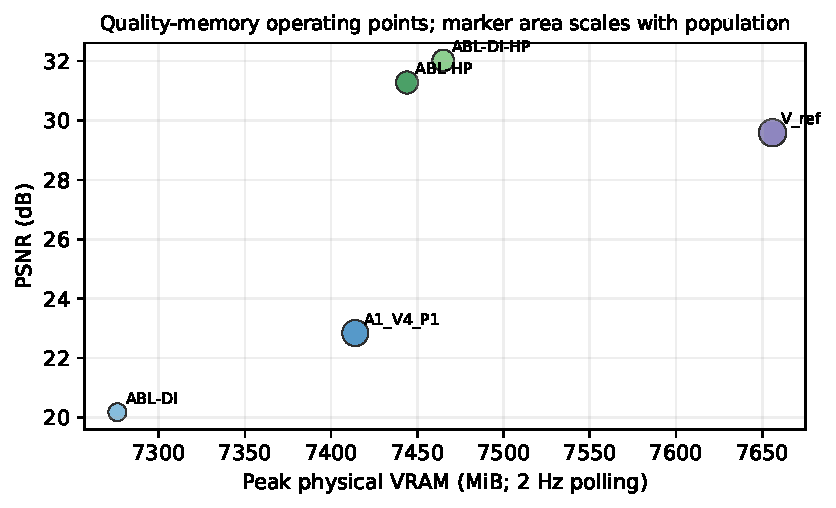
\includegraphics[width=\columnwidth]{figures/fig4_quality_memory.pdf}
\caption{Bonsai seed-0 operating points. Marker area scales with final Gaussian count; whole-device peak VRAM is not monotonic in population.}
\label{fig:qmem}
\end{figure}

\subsection{Factorial Ablation}
Table~\ref{tab:factorial} and Fig.~\ref{fig:factorial} give the complete seed-0 factorial grid. Averaging over inflow policies, preservation contributes $+10.1432$ dB PSNR, $+0.2179$ SSIM, and $-0.2600$ LPIPS. Averaging over lifecycles, dynamic inflow contributes $+0.9605$ dB. The interaction is substantial: dynamic rather than static inflow changes PSNR by $+2.6660$ dB under eager hygiene but by $-0.7451$ dB under preservation, a difference-in-differences of $-3.4111$ dB. Hence the inflow main effect should not be interpreted independently of lifecycle.

\begin{table*}[t]
\centering\scriptsize
\caption{Full 2x2 factorial ablation on Bonsai, seed 0. Each cell is one physical run.}
\label{tab:factorial}
\begin{tabular}{llccccc}
\toprule
Inflow & Lifecycle & PSNR $\uparrow$ & SSIM $\uparrow$ & LPIPS $\downarrow$ & Gaussians & Peak MiB\\
\midrule
Static 5K & Eager hygiene & 20.1739 & .7044 & .4691 & 358,651 & 7,276\\
Dynamic 5K--15K & Eager hygiene & 22.8399 & .7430 & .3975 & 1,106,240 & 7,414\\
Static 5K & Preserve & \textbf{32.0227} & \textbf{.9456} & \textbf{.1618} & 653,344 & 7,465\\
Dynamic 5K--15K & Preserve & 31.2776 & .9376 & .1737 & 705,392 & 7,444\\
\bottomrule
\end{tabular}
\end{table*}

\begin{figure}[t]
\centering
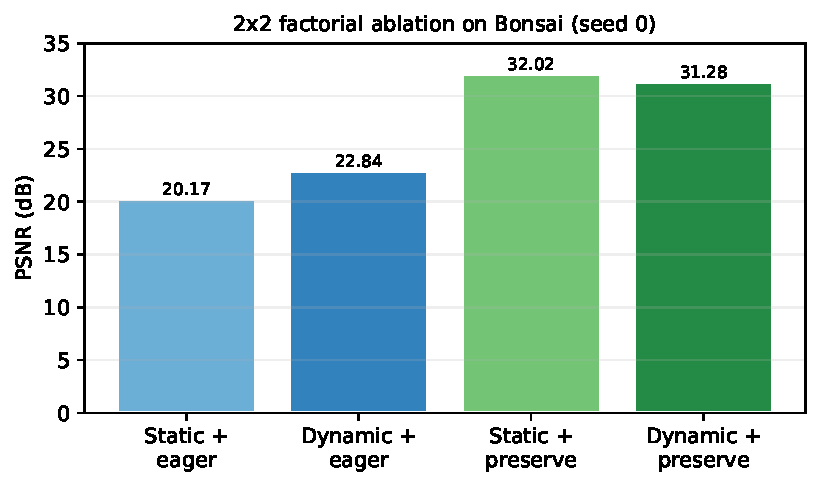
\includegraphics[width=\columnwidth]{figures/fig3_factorial.pdf}
\caption{Lifecycle dominates the seed-0 factorial result; dynamic inflow helps only under eager hygiene in this grid.}
\label{fig:factorial}
\end{figure}

\subsection{Cross-Scene Evaluation}
Preservation improves all three tested scenes relative to the matching memory-bounded baseline (Table~\ref{tab:crossscene}). Garden gains 6.2543 dB, $+0.3608$ SSIM, and $-0.3645$ LPIPS; Flowers gains 2.9422 dB, $+0.1793$ SSIM, and $-0.1846$ LPIPS. These are paired seed-0 observations. Only Bonsai has multi-seed replication.

\begin{table}[t]
\centering\scriptsize
\caption{Cross-scene seed-0 results (baseline $\rightarrow$ preservation).}
\label{tab:crossscene}
\begin{tabular}{lccc}
\toprule
Scene & PSNR & SSIM & LPIPS\\
\midrule
Bonsai & $22.84\!\rightarrow\!31.28$ & $.743\!\rightarrow\!.938$ & $.397\!\rightarrow\!.174$\\
Garden & $18.67\!\rightarrow\!24.93$ & $.385\!\rightarrow\!.746$ & $.674\!\rightarrow\!.310$\\
Flowers & $17.36\!\rightarrow\!20.30$ & $.338\!\rightarrow\!.517$ & $.651\!\rightarrow\!.466$\\
\bottomrule
\end{tabular}
\end{table}

\begin{figure}[t]
\centering
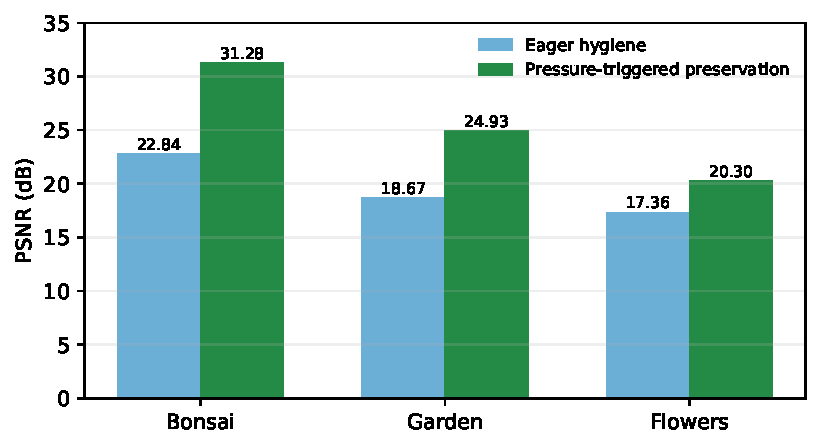
\includegraphics[width=\columnwidth]{figures/fig5_cross_scene.pdf}
\caption{Seed-0 PSNR across the three evaluated Mip-NeRF 360 scenes.}
\label{fig:crossscene}
\end{figure}

\subsection{Memory and Quality--Memory Trade-off}
All 24 audited physical runs complete with exit code zero and no recorded OOM. Sampled peaks span 6,906--7,656 MiB, leaving at least 494.56 MiB relative to the reported 8,150.56-MiB capacity. For the proposed seed-0 runs, Bonsai, Garden, and Flowers peak at 7,444, 7,570, and 7,288 MiB, respectively. Garden preservation increases population from 336,391 to 580,115 while reducing the sampled peak by 86 MiB; Flowers preservation reduces population from 707,777 to 426,905 while increasing the peak by 346 MiB. External WDDM use, rasterization buffers, timing, and allocator fragmentation therefore dominate any simple count-to-physical-memory relation.

\begin{table}[t]
\centering\scriptsize
\caption{Memory efficiency of seed-0 preservation runs. Headroom is capacity minus sampled peak.}
\label{tab:memory}
\begin{tabular}{lrrr}
\toprule
Scene & Gaussians & Peak MiB & Headroom MiB\\
\midrule
Bonsai & 705,392 & 7,444 & 706.56\\
Garden & 580,115 & 7,570 & 580.56\\
Flowers & 426,905 & 7,288 & 862.56\\
\bottomrule
\end{tabular}
\end{table}

The internal telemetry trace (supplementary Fig.~S1) remains below the controller's 5,632-MiB effective budget in the shown runs. This does not imply that total physical VRAM follows the same curve; the quantities have different scopes.
